\chapter{Vergleich zwischen Docker Swarm und Kubernetes}\label{ch:comparison}

Wie eingangs bereits erw\"ahnt, ist Docker Swarm nicht die einzige Software zur Containerorchestrierung.
Neben anderen Alternativen gibt es Kubernetes, das nicht nur bekannter und weiter verbreitet ist, sondern inzwischen auch direkt in Docker Desktop integriert ist und den Industriestandard darstellt. 
Ohne zu tiefgreifend auf die Architektur und Funktionsweise von Kubernetes einzugehen, soll dennoch im Folgenden ein Vergleich zwischen den beiden Optionen gewagt werden.

\begin{figure}[h]
    \centering
    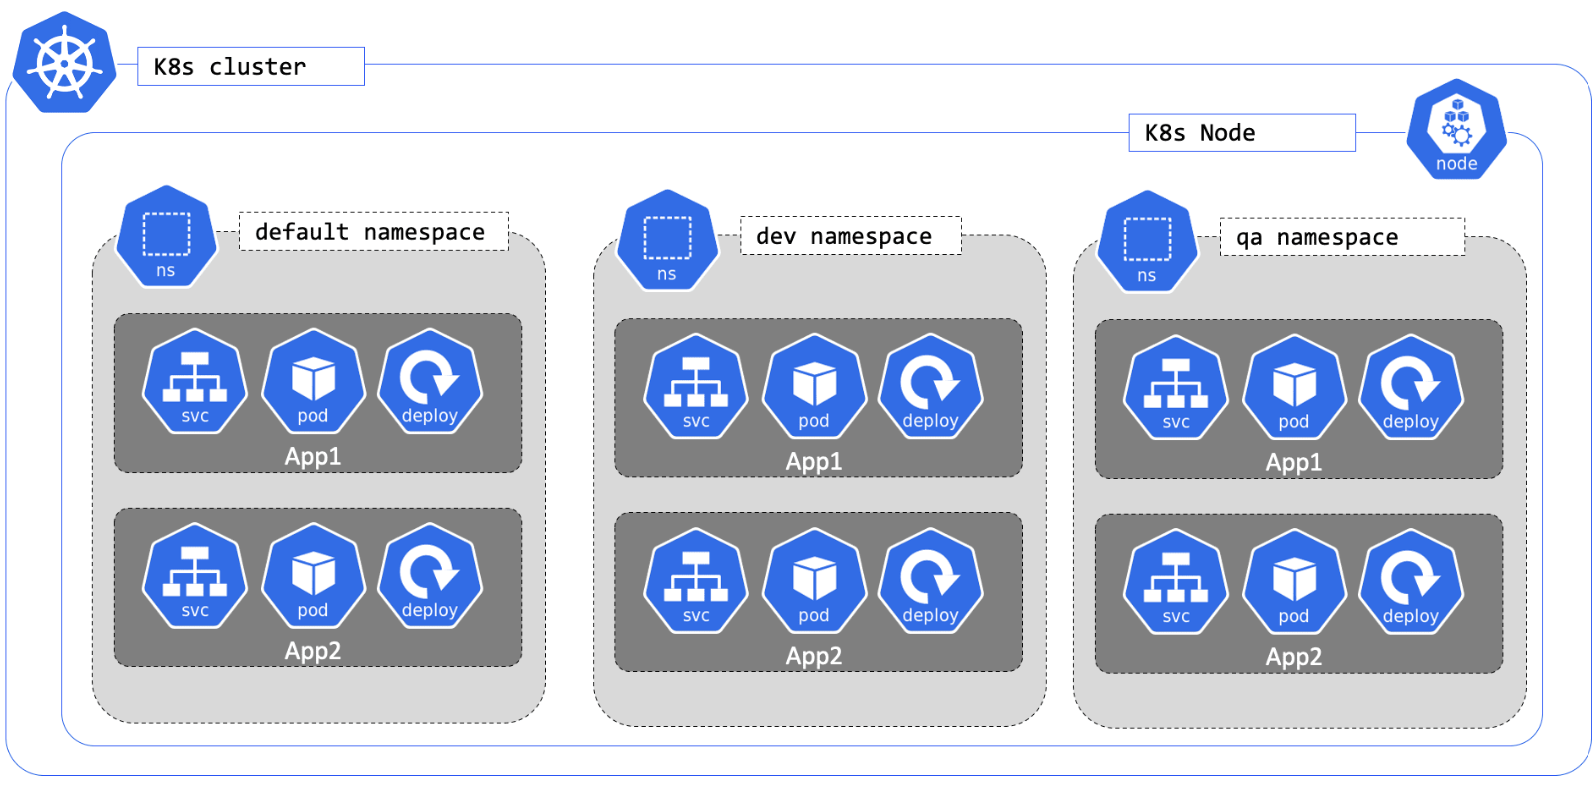
\includegraphics[width=0.7\textwidth]{figures/kubernetes.png}
    \caption{\"Ubersicht des architektonischen Aufbaus eines Kubernetes-Clusters\cite{kumar_working_2019}}
    \label{fig:k8s-cluster}
\end{figure}

In den Grundfunktionalit\"aten unterscheiden die beiden Orchestrierungssoftwares sich wenig. 
Sie beinhalten gleicherma{\ss}en Funktionen, um Docker Container zu starten, zu stoppen, deren Verf\"ugbarkeit zu kontrollieren und auf Ausf\"alle zu reagieren. 
Ebenso bieten beide Systeme Optionen zur Lastverteilung und Ressourcenverwaltung des Host-Systems. 
Dadurch k\"onnen z.B.\ Container automatisiert von einem System auf ein anderes im gleichen Cluster umgezogen werden, sofern ein Cluster Fehler wirft oder nicht mehr gen\"ugend Ressourcen bereitstellen kann. 

In der Art und Weise wie Skalierung gehandhabt wird, treten aber schon die ersten Unterschiede auf. 
Skalierung bezeichnet das Replizieren von Containern, um eine h\"ohere Last aufzufangen.
Bei Docker Swarm muss die Anzahl an Replikas immer manuell angegeben werden, entweder wie oben gezeigt \"uber die Compose-Datei, im Nachhinein durch einen Docker-Befehl oder eine separate UI wie bspw.\ Portainer. 
In Kubernetes hingegen ist es m\"oglich festzulegen, dass bspw.\ ab einer bestimmten Auslastung automatisch zus\"atzliche Container in sogenannten Pods gestartet werden. 
Dies geschieht mittels des Horizontal Pod Autoscalers (HPA), der ``die Anzahl der Pods in einem Deployment oder Replica Set basierend auf beobachteten CPU-Auslastung oder anderen ausgewählten Metriken automatisch skaliert''.\cite{briegel_kubernetes_2023}
Dies wird unterst\"utzt durch den Vertical Pod Autoscaler und den Cluster Autoscaler, die zus\"atzliche Skalierungsoptionen bieten.\cite{briegel_kubernetes_2023}

Ein Aspekt, der inbesondere im Kontext von cloud-basierten Anwendungen relevant ist, ist die Sicherheit. 
Hier bieten beide Systeme ihre eigenen L\"osungen an, wenn auch auf unterschiedliche Art und Weise. 
Der Netzwerkverkehr zwischen Containern ist in Docker Swarm standardm\"a{\ss}ig verschl\"usselt, um Man-in-the-Middle-Angriffe oder \"ahnliches zu verhindern. 
Dar\"uber hinaus stellt Docker Swarm grundlegende Funktionalit\"aten zur Verwaltung von Secrets zur Verf\"ugung. 
W\"ahrend diese Funktionen ohne Frage wichtig sind, sind bei Docker Swarm  die Konfigurationsoptionen diesbez\"uglich beschr\"ankt.

Das ist einer der Punkte, aufgrund dessen Kubernetes in vielen F\"allen bevorzugt wird. 
Nicht nur bietet Kubernetes diese beiden und mehr Funktionen an, sondern gibt den Userinnen auch mehr M\"oglichkeiten, bspw.\ Netzwerkrichtlinien auf der Ebene von Pods zu erstellen.\cite{briegel_kubernetes_2023}
